\documentclass{ximera}

\newcommand{\RR}{\mathbb R}
\renewcommand{\d}{\,d}
\newcommand{\dd}[2][]{\frac{d #1}{d #2}}
\renewcommand{\l}{\ell}
\newcommand{\ddx}{\frac{d}{dx}}
\newcommand{\dfn}{\textbf}
\newcommand{\eval}[1]{\bigg[ #1 \bigg]}


\author{Jim Talamo}
\license{Creative Commons 3.0 By-NC}


\outcome{Review integration techniques}


\begin{document}
\begin{exercise}
 Consider the initial value problem (IVP) $\frac{dy}{dx} = \frac{-8xe^{2x}}{y}, ~ ~ ~ ~ y(0)=-1.$

%\item[I.] [3 pts] Sketch the solution to the IVP on the direction field below.
%
% \begin{figure}[h!]
% \centering
%  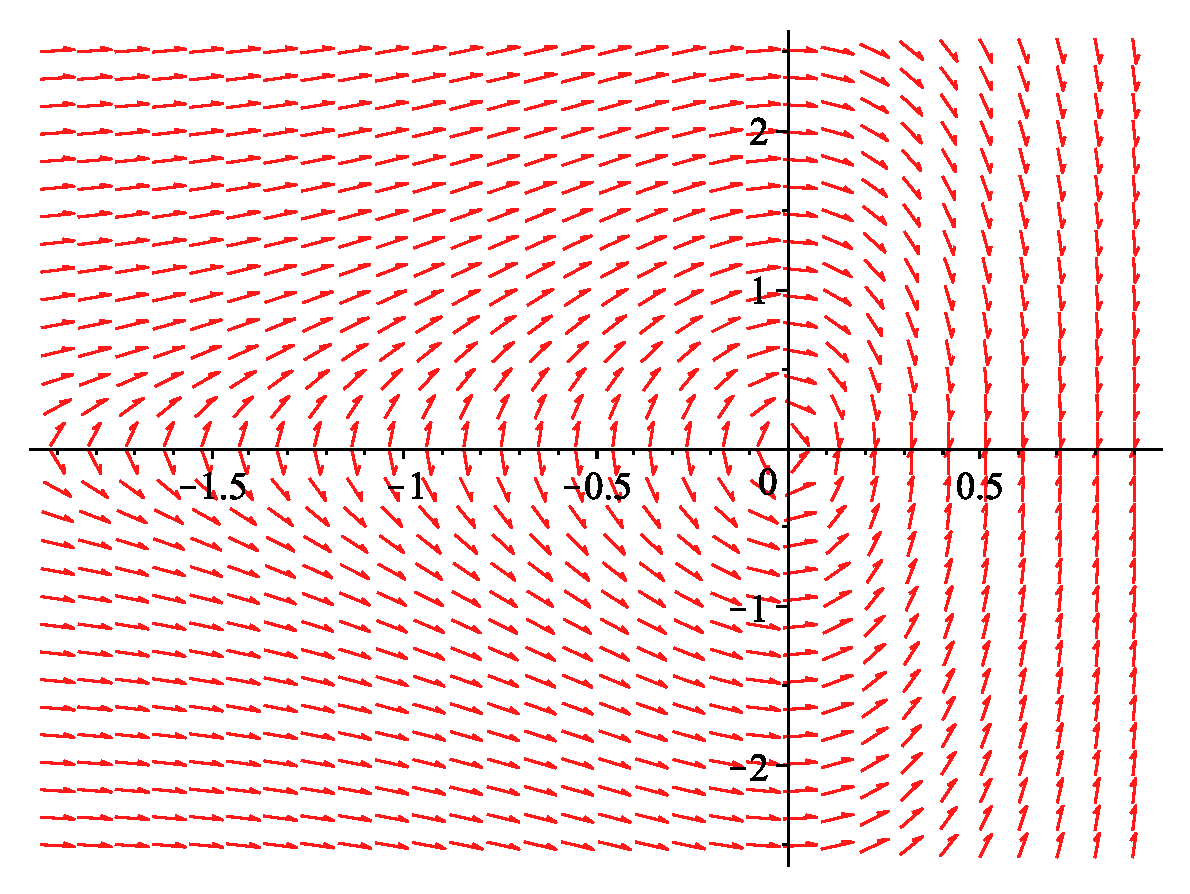
\includegraphics[width=.5 \textwidth]{IVP.eps}
%\end{figure}
%
%Based on the direction field, it looks like the solution is defined for $\underline{\hspace{15mm}} \leq x \leq \underline{\hspace{15mm}}$.
%
%\vspace{3mm}
%
%\item[II.] [9 pts] Solve the initial value problem $\frac{dy}{dx} = \frac{-8xe^{2x}}{y}, ~ ~ ~ ~ y(0)=-1.$.  Explicitly solve for $y$ in your final answer.  
%
%\vspace{70mm}
%
%\item[III.] [2 pts] Write down an inequality in $x$ that gives the domain of the solution.  You do not need to solve the inequality.
%
%\newpage

%%%MAKE THEM USE TAYLOR POLYNOMIAL TO APPROXIMATE DOMAIN FOR a=-1

%%%Make THEM FIND smallest a SOL SOLUTION CAN BE EXTENDED BACKAWRDS FOR ALL TIME

\end{exercise}
\end{document}
